\documentclass{beamer}
%\usetheme{Ilmenau}
%\usecolortheme{beaver}

\usepackage[slovak,american]{babel}
\usepackage[utf8]{inputenc}
\usepackage{graphicx}
\usepackage{adjustbox}

 \usepackage{xcolor}
 
 \newsavebox\MBox
\newcommand\Cline[2][red]{{\sbox\MBox{$#2$}%
  \rlap{\usebox\MBox}\color{#1}\rule[-2.2\dp\MBox]{\wd\MBox}{1pt}}}

%\usefonttheme{serif}

%\definecolor{UKOrange}{HTML}{ef9424} %
\definecolor{UKOrange}{HTML}{7a2c18} %
\definecolor{UKBrown}{HTML}{a96d5e} %
\definecolor{UKLight}{HTML}{d8b6ab} %
\definecolor{UKDark}{HTML}{7a4f44}
\definecolor{UKDarker}{HTML}{4d312b} 
\definecolor{UKDarkest}{HTML}{2e1e1a}
\definecolor{UKRed}{HTML}{bf1f1c}

\setbeamertemplate{footline}[frame number]{}
\setbeamertemplate{navigation symbols}{}

%\usecolortheme{beaver}
\setbeamertemplate{itemize item}[square]
\setbeamercolor{itemize item}{fg = UKBrown}
\setbeamercolor{itemize subitem}{fg = UKLight}
\setbeamercolor{enumerate item}{fg = UKDark}

\setbeamercolor{footnote}{fg=UKLight}
\setbeamercolor{footnote mark}{fg=UKLight}
\setbeamerfont{footnote}{size=\tiny}
\renewcommand\footnoterule{}

\usetheme{default}
\beamertemplatenavigationsymbolsempty
\setbeamercolor{title}{fg=white, bg=UKBrown}
\setbeamercolor{frametitle}{fg=white, bg=UKBrown}
\setbeamercolor{block title}{bg=UKBrown, fg= white}
\setbeamercolor{block body}{bg =UKLight, fg = UKDarkest}

\setbeamercolor{block title alerted}{bg=UKOrange, fg= white}
\setbeamercolor{block body alerted}{bg =UKLight, fg = UKDarkest}


%\setbeamercolor{section in toc}{fg = UKBrown}
%\setbeamercolor{section in toc}{fg = UKDarkest}

% odstrani gulicky
\renewcommand*{\slideentry}[6]{}

\useoutertheme[subsection=false]{miniframes}
\AtBeginSection[]{\subsection{}}

\setbeamercolor{below lower separation line head}{bg=UKDark}
\addtobeamertemplate{headline}{}{%
  \begin{beamercolorbox}[colsep=0.5pt]{below lower separation line head}
  \end{beamercolorbox}
}
%\setbeamercolor*{mini frame}{fg=white,bg=UKRosy}
\setbeamercolor{section in head/foot}{fg=UKLight, bg=UKDark}

\usepackage{etoolbox}
\makeatletter
\preto{\@verbatim}{\topsep=0pt \partopsep=0pt }
\makeatother

%\setbeamertemplate{itemize/enumerate body begin}{\normalsize}
%\setbeamertemplate{itemize/enumerate subbody begin}{\normalsize}




%\newcommand{\codeblock}[2]{ \begin{block}{#1} \begin{verbatim}#2\end{verbatim}\end{block}}

%\defbeamertemplate*{title page}{customized}[1][]
%{
%  \begin{centering}
%    \begin{beamercolorbox}[sep=8pt,center]{title}
%      \usebeamerfont{title}\inserttitle
%    \end{beamercolorbox}
%  \end{centering}
%  \bigskip
%
%\begin{columns}[onlytextwidth,T]
%
%
%  \column{27mm}
%  \includegraphics[width=27mm]{images/logoFMFI.png}
%  
%  \column{\dimexpr\linewidth-54mm-6mm}
%  \centering
%  \vspace{5mm}  
%  \usebeamerfont{author}\insertauthor\par
%  \vspace{5mm}
%  \usebeamerfont{institute}\insertinstitute\par
%
%  \column{27mm}
%  \includegraphics[width=27mm]{images/logoUK.png}  
%\end{columns}
%\centering
%\vspace{7mm}
%  \usebeamerfont{date}\insertdate\par
%}

\DeclareMathOperator*{\argmin}{arg\,min}
\newcommand{\e}[1]{$\cdot 10^{#1}$}
\newcommand*\mean[1]{\bar{#1}}

\newcommand*{\Z}{\mathbb{Z}}

%\newcommand{\codeblock}[2]{ \begin{block}{#1} \begin{verbatim}#2\end{verbatim}\end{block}}



\title[8. cvičenie]{Pokročilé spracovanie obrazu - Morfológia II.}
\author[Kocur]{Ing. Viktor Kocur \\{\small viktor.kocur@fmph.uniba.sk}}
\institute{DAI FMFI UK}
\date{13.11.2018}

\begin{document}
\selectlanguage{slovak}

\begin{frame}
  \titlepage
\end{frame}

\section{Binárne obrazy}
\subsection{Granulometria}

\begin{frame}
\frametitle{Granulometria}
  \begin{block}{Otvorenie s rôznymi SE}
  Ak binárny obraz otvárame postupne väčšími štruktúrnymi elementmi môžeme dostať informáciu o distribúcii veľkosti objektov.
  \end{block}
  

  \begin{block}{Úloha}
  Otvárajte obrázok granulometria.png postupne väčšími štruktúrnymi elementmi. Zobrazte graf na ktorom bude vidieť vzťah medzi obsahom otvoreného obrazu a veľkosťou štruktúrneho elementu.
  \end{block}
\end{frame}

\subsection{Podmienaná dilatácia}

\begin{frame}
\frametitle{Podmienená dilatácia}
  \begin{block}{Podmienená dilatácia - definícia}
  Obraz prahujeme dvoma prahmi. Dostaneme dva obrazy $A$ pre vyšší prah a $B$ pre nižší. Podmienená dilatácia so štruktúrnym elementom $SE$ je potom $(A \oplus SE) \cap B$.
  \end{block}  

  \begin{block}{Úloha}
  Otestujte podmienenú dilatáciu pre obrázok bunky.png.
  \end{block}
\end{frame}

\section{Šedotónová morfológia}

\subsection{Morfologické operácie}

\begin{frame}
\frametitle{Erózia a dilatácia pre šedotónový obraz} 

  \begin{block}{Dilatácia a erózia}
  Pre $f, h \colon \mathbb{R}^2 \to \mathbb{R}$ s konečnými nosičmi platí $f \oplus h = max\{ f(x-r, y-s) + h (r,s) | (r,s) \in supp(h)\}$ a \\
  $f \ominus h = min\{ f(x-r, y-s) - h (r,s) | (r,s) \in supp(h)\}$
  \end{block}   

  \begin{block}{Matlab}
  Morfologické príkazy v matlabe fungujú aj pre šedotónové obrazy.
  \end{block}
  
  \begin{block}{Úloha}
  Otestujte si dilatáciu, eróziu, otvorenie a zatvorenie na obrázku zátišie.pgm. Použite zatvorenie a následné otvorenie na vyhladenie obrazu.
  \end{block}   
\end{frame}


\subsection{Morfologický gradient}

\begin{frame}
\frametitle{Morfologický gradient} 

  \begin{block}{Morfologický gradient}
  $grad(I) = \frac{(I \oplus SE) - (I \ominus SE)}{2}$
  \end{block}   

  \begin{block}{Morfologický gradient - interný}
  $grad(I) = I - (I \ominus SE)$
  \end{block}     
  
  \begin{block}{Morfologický gradient - externý}
  $grad(I) = (I \oplus SE) - I$
  \end{block}     
  
  \begin{block}{Úloha}
  Otestujte detekciu hrán pomocou morfologického gradientu.
  \end{block}   
\end{frame}

\subsection{Top a Bottom-hat}

\begin{frame}
\frametitle{Top-hat a bottom-hat transformácia} 

  \begin{block}{Top-hat transformácia}
  Top-hat transformácia je rozdiel originálneho obrazu a jeho otvorenia. Bottom-hat transformácie je rozdiel uzavretia obrazu a jeho originálu. 
  \end{block}  
  
  \begin{block}{imtophat}
  imtophat(I, SE) - vráti obraz po top-hat transformácii štruktúrnym elementom SE
  \end{block}    
  
  \begin{block}{imbothat}
  imbothat(I, SE) - vráti obraz po bottom-hat transformácii štruktúrnym elementom SE
  \end{block}      
\end{frame}

\begin{frame}
\frametitle{Adaptívna segmentácia} 

  \begin{block}{Segmentácia na nekonštantnom pozadí}
  Top-hat transformáciu môžeme použiť na segmentáciu svetlých objektov na nekonštantnom pozadí. Bottom-hat môžeme použiť na segmentáciu tmavých objektov.
  \end{block}  
  
  \begin{block}{Úloha}
  Segmentujte qr kódy z qr.png a ryžu z rice.png.
  \end{block}    
\end{frame}

\begin{frame}
\frametitle{Úprava kontrastu} 
  \begin{block}{Zvýšenie kontrastu}
  V obraze môžeme zvýšiť kontrast pomocou pričítania top-hat transformácie a odpočítania bottom-hat transformácie od originálu.
  \end{block} 
  
  \begin{block}{Úloha}
  Zvýšte kontrast v obrázku krajinka.png.
  \end{block}          
\end{frame}

\subsection{Rekonštrukcia}

\begin{frame}
\frametitle{Rekonštrukcia}
\begin{center}
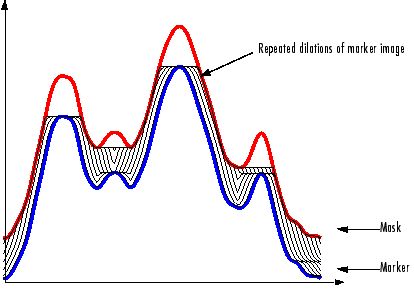
\includegraphics[width= 0.8\textwidth]{recon.png}
\end{center}
\end{frame}


\begin{frame}
\frametitle{Rekonštrukcia}
\begin{center}
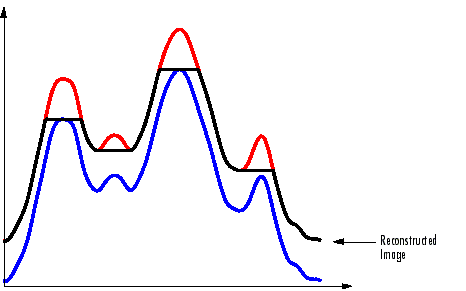
\includegraphics[width= 0.8\textwidth]{recon2.png}
\end{center}
\end{frame}

\begin{frame}
\frametitle{Rekonštrukcia}

  \begin{block}{Vyplnenie vybraného objektu}
  Rekonštrukciou môžeme v binárnom obraze (mask) segmentovať vybrané objekty. Ak ako tzv. marker vyberieme binárny obraz do ktorého patria nejaké body, tak rekonštrukciou vyplníme iba tie oblasti s ktorými sú tieto body spojené.
  \end{block}  
  
  \begin{block}{imreconstruct}
  imreconstruct(marker, mask) - vráti rekonštrukciu maky podľa markera.
  \end{block}  
  
  \begin{block}{Úloha}
  Použite ginput a segmentujte iba to písmeno z text.png, na ktoré uživateľ klikne.
  \end{block}  

\end{frame}



\end{document}